The chapter outlines the hardware testing procedures for the Single Chip Mote digital system. Unit-level testbenches and simulation are used to verify that modules or small groups of modules behave properly in isolation; real-time tests on the FPGA hardware indicate that the entire system works together as expected, including interfaces with the analog and radio circuits. Mistakes in the final ASIC version of this chip are extremely costly, and simulating the entire Single Chip Mote in Cadence or Synopsys is computationally intensive and slow. Therefore, it is essential that the Single Chip Mote digital system is thoroughly tested in simulation and on an FPGA before moving on to an ASIC design.

\section{Simulation Testing Using ISim}
New Verilog modules and major changes to existing modules should be verified in simulation to catch any bugs before integrating the module into the Single Chip Mote digital system. While it is difficult to simulate the entire Single Chip Mote digital system altogether, designers typically use unit-level tests to check that modules are functioning correctly and low-level integration tests to ensure that combinations modules work together and interface as expected. The module or modules being tested are referred to as the device under test (DUT) or unit under test (UUT). Xilinx ISE uses a Verilog simulator, called ISim, to simulate testbenches added to an ISE project.

\subsection{Original Testbenches for Spartan 6}
The Single Chip Mote digital system was originally designed by Francesco Bigazzi, a visiting scholar, for the Spartan 6 FPGA. Bigazzi created separate ISE projects for each testbench, with separate folders to hold the testbench and DUT Verilog code. Note that Bigazzi used a copy of the DUT Verilog code for his testbenches, rather than linking to the original files that are used for the implementation. Thus any corrections made while testing needed to be copied back to the original file. Each ISE project and its accompanying code are saved in their own folder in \path{scm-digital/proj/ise/spartan6/testbench/TESTs}. For example, the \path{scm-digital/proj/ise/spartan6/testbench/TESTs/ADC} folder contains the \path{ADC.xise} project file for testing Bigazzi's original ADC controller implementation. The \path{scm-digital/proj/ise/spartan6/testbench/TESTs/ADC/src} folder contains a copy of Bigazzi's original ADC code and any additional testbench code.

Many of the testbenches in the \path{scm-digital/proj/ise/spartan6/testbench/TESTs} folder are outdated since modules have been deprecated and are no longer in use (such as the original ADC controller and the original AHB arbiter). Also, there is no coherency between the code in \path{scm-digital/src/hw/spartan6} and the code stored for each individual test. Modules have been updated during the course of the project while their testbenches (and the copies of the DUT modules) have not. For example, the \texttt{APBMUX} module has been modified to add and remove APB peripherials, and the testbench designed by Bigazzi is not compatible. The \texttt{Rfcontroller} module went through a large revision to add the spreader and correlator/despreader module, to add an interface to the radio timer, and to improve the memory-mapped register interface. Therefore the original testbench, which verified the TX and RX state machines before these changes, is now incompatible. This does not mean that these changes went untested, as individual testbenches were created to verify the spreader, correlator/despreader, and radio timer. The integration of these modules was verified in real-time on the FPGA rather than through testbenches. However, this is not the best practice nor is it an accurate reflection of the testing procedure used in industry, and further care must be taken in the future to ensure that all non-trivial changes are verified.

\subsection{Artix 7 Testbenches and Improved Testing Procedure}
With the transition from the Spartan 6 to Artix 7 FPGA, and the accompanying changes to the git repo and file organization, a new testing procedure is devised to ensure greater coherency between the module code and their testbenches.

There is a single ISE project, \texttt{scm-digital/proj/ise/artix7/testbench/te\-s\-t\-b\-ench.xise}, for all new testbenches. The code for the testbenches themselves are found in the \path{scm-digital/src/hw/artix7/uRobotDigitalController/testbench} folder, while the code for the device under test is the same as the implementation code, found in \path{scm-digital/src/hw/artix7/uRobotDigitalController}. Therefore, any changes or corrections made during simulation testing are applied to the actual code for the module, rather than a copy of that module's code. Any changes or corrections made while testing with the FPGA in real-time should be verified by running the testbenches again (without the need for copying since the same code is used for simulation and implementation). Any major revisions require that the testbench code is updated alongside with the DUT code, and that the new tests pass in simulation before verifying in real-time.

The ISE project for testbenches, \path{scm-digital/proj/ise/artix7/testbench/testbench.xise}, currently has 5 testbenches:

\begin{description}
	\item[RFTIMER\_tb] Tests the radio timer module \texttt{RFTIMER}. The compare and capture units are configured and then the timer is enabled. Stimulus is applied to the DUT and the testbench ensures that it behaves as expected.
	\item[SFD\_delay\_TB] Tests how long (in time) it takes to send the last bit of the SFD of a packet after telling the radio controller to send a packet (using \texttt{TX\_SEND}). Also test how long (in time) it takes to send the last bit of a packet after telling the radio controller to send a packet. This testbench use a clock frequency of 2MHz, to match the implementation. Example packet data is loaded into the \texttt{tx\_fifo2} module connected to the \texttt{spreader} module. The \texttt{spreader} module is then activated using the \texttt{tx\_start} input and the testbench runs until the \texttt{tx\_sfd\_sent} and \texttt{done} outputs are asserted. The time between \texttt{tx\_start} and \texttt{tx\_sfd\_sent} is calculated along with the time between \texttt{tx\_start} and \texttt{done}.
	\item[LOAD\_delay\_TB] Tests how long (in time) it takes in the worst-case to copy packet data into the TX FIFO for radio transmission. This is the time between when the \texttt{TX\_LOAD} signal activates the radio controller, and when the radio controller indicates it is done using the \texttt{TX\_LOAD\_DONE} interrupt. This testbench uses a clock frequency of 5MHz, to match the implementation. The \texttt{RFcontroller}, \texttt{AHBDMEM}, \texttt{DMA\_V2}, \texttt{AHBLiteArbiter\_V2}, and AHBsub bus modules are required for this experiment. In order to replicate the worst-case scenario, the largest possible packet (127 bytes) is loaded into the TX FIFO while the Master 0 input of the arbiter (which is used for the Cortex-M0) is always requesting access to the AHBsub bus. This way the DMA must wait each time it tries to copy data from the data memory to the radio controller.
	\item[correlator\_TB] Tests the \texttt{corr\_despreader} and \texttt{correlator} modules to ensure that they can detect and return a packet using an input data stream from an MSK demodulator. An example data stream of MSK chips is clocked into the \texttt{corr\_despreader} module, which converts it to packet data on the \texttt{dout} output. The output is then compared with the actual packet data that corresponds to the input MSK chips.
	\item[spreader\_TB] Tests the combination of the \texttt{tx\_fifo2}, \texttt{spreader}, \texttt{symbol2chips}, \texttt{correlator}, \texttt{corr\_despreader}, and \texttt{rx\_fifo} modules. Regular packet data is loaded into the \texttt{tx\_fifo2} module. The \texttt{spreader} module reads it out and converts it to a serial data stream for an MSK modulator (using the \texttt{symbol2chips} module). The \texttt{corr\_despreader} module reads that data stream (assuming it came from an MSK demodulator) and converts it back to regular packet data (using the \texttt{correlator} module) which is then stored into the \texttt{rx\_fifo} module. This simulates sending and receiving a packet, and if the data in the two FIFOs match then the modules are operating correctly.
\end{description}

As the Single Chip Mote digital system is expanded and modified, more testbenches should be added to the ISE project and all changes should be verified in simulation.

\subsection{Using ISim}
To simulate a testbench using ISim, first open an ISE project containing a testbench, such as \path{scm-digital/proj/ise/artix7/testbench/testbench.xise}. In the Design Hierarchy panel, select the Simulation view (as shown in Figure \ref{fig:isim-load-ise2}) to see a list of all the testbenches in the project. Selecting one of these testbenches brings up the Simulate Behavioral Model process in the Process panel. Running this process compiles the testbench and Verilog code into an executable and launches ISim to run that executable. Before simulating, it is recommended that the settings for the Simulate Behavioral Model process are modified to match the current testbench. Right-clicking the Simulate Behavioral Model and selecting Process Properties... (as shown in Figure \ref{fig:isim-load-ise2}) brings up the ISim Properties window (Figure \ref{fig:isim-properties2}).

The first property to modify is the Simulation Run Time. The default run time (when the Run for Specified Time box is unchecked) is 1000ns. For large testbenches, the default time is too short and the simulation pauses in the middle of the test (the console can be used in ISim to manually direct the simulation to continue). Therefore the Simulation Run Time should be set to some time larger than the total run time of the testbench. This can be estimated by taking the time unit value (specified using the \texttt{`timescale} directive at the top of every testbench) and multiplying it by the number of time steps executed. For example, the following code sets the time unit to 1ns: \texttt{`timescale 1ns / 1ps}, and the following line executes 12 time steps: \texttt{\#12;}. The Simulation Run Time parameter should not be too large in order to avoid simulating longer than needed. Another alternative is to make the Simulation Run Time parameter much larger than necessary, and then adding \texttt{\$finish;} to the end of the testbench to stop execution exactly when the test completes.

The second property to modify is the Custom Waveform Configuration File. A waveform configuration file is used by ISim to display signals from the testbench in the waveform window. When no waveform configuration file is specified, ISim by default displays the waveforms of the top-level signals in the testbench. Waveforms for signals inside of the DUT and other instantiated modules can be added to the waveform window; however, the simulation must be run again in ISim (using the \texttt{restart} and \texttt{run} commands in the console) in order for the waveforms to display properly. If ISim is closed and re-opened, such as when the Verilog code is modified and re-compiled, all of the non-default waveforms must be added again. When a waveform configuration file is specified, ISim will automatically add all of the waveforms before executing the simulation. Therefore, the recommended approach is to run a testbench without a waveform configuration file, add all of the signals of interest to the waveform window, save the waveform configuration, and then modify the Custom Waveform Configuration File property. When using ISim, more signals can be added to the waveform view and saved to the same waveform configuration file; the new signals will also be added automatically the next time ISim is opened. Each testbench should have its own waveform configuration file, and the Custom Waveform Configuration File property must be changed when switching between testbenches.

\begin{figure}
\centering
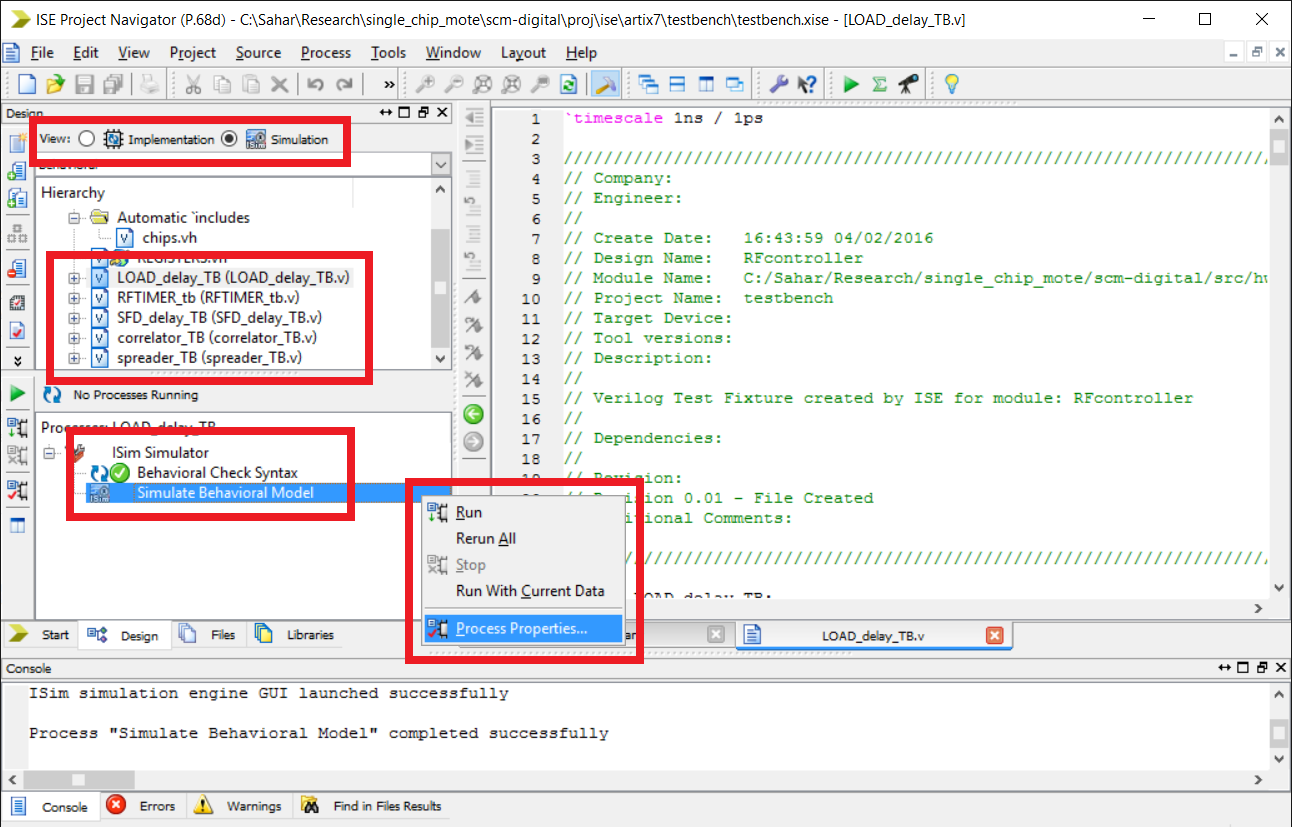
\includegraphics[width=1\linewidth]{isim-load-ise2}
\caption{Running a simulation in ISE}
\label{fig:isim-load-ise2}
\end{figure}

\begin{figure}
\centering
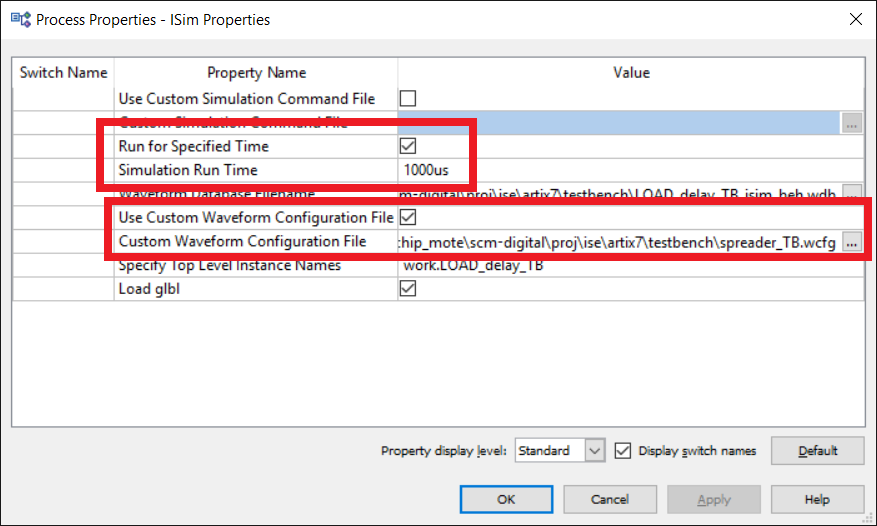
\includegraphics[width=1\linewidth]{isim-properties2}
\caption{ISim Properties window}
\label{fig:isim-properties2}
\end{figure}

Figure \ref{fig:isim-waveform0}-\ref{fig:isim-waveform3} demonstrate how to add signals to the waveform window, restart and run the simulation using the console, and save a wave configuration file to be used for later simulations. Figure \ref{fig:isim-waveform0} shows the ISim window after launching a simulation using the default wave configuration file. The console shows all \texttt{\$display} and other varieties of print statements. The console also shows that the simulation stopped after 110100ns; this is due to the \texttt{\$finish;} line added to the end of the testbench code. Otherwise, the simulation would have continued to run until it reached the value specified by the Simulation Run Time parameter. The waveform window by default shows the waveforms of all the top-level signals. Most of these signals are not necessary and can be removed. The order of these signals can also be re-arranged, and the radix used to display the values of each bus can be changed.

To add more signals to the waveform window, first click on the module or process that contains that signal in the Instance and Process panel on the left side of the ISim window. This updates the Objects panel to list all of the signals inside of that module or process. Right-clicking a particular signal and selecting Add To Wave Window (or dragging the signal into the window) adds the waveform. These steps are shown in Figure \ref{fig:isim-waveform1}.

Once the waveform window is updated with the required signals, the console can be used to restart and run the simulation again to plot all of the waveforms. This is show in Figure \ref{fig:isim-waveform2}. When a simulation is paused (for example at time 100ns), more signals can be added to the waveform window; however, their waveforms for all time steps before 100ns will not be displayed. If the simulation is continued after that point (by using the \texttt{run} command in the console), the waveform for all time steps after 100ns will be displayed.

Figure \ref{fig:isim-waveform3} shows how to save the waveform configuration file using the Save As... option in the File menu.

\begin{figure}
	\centering
	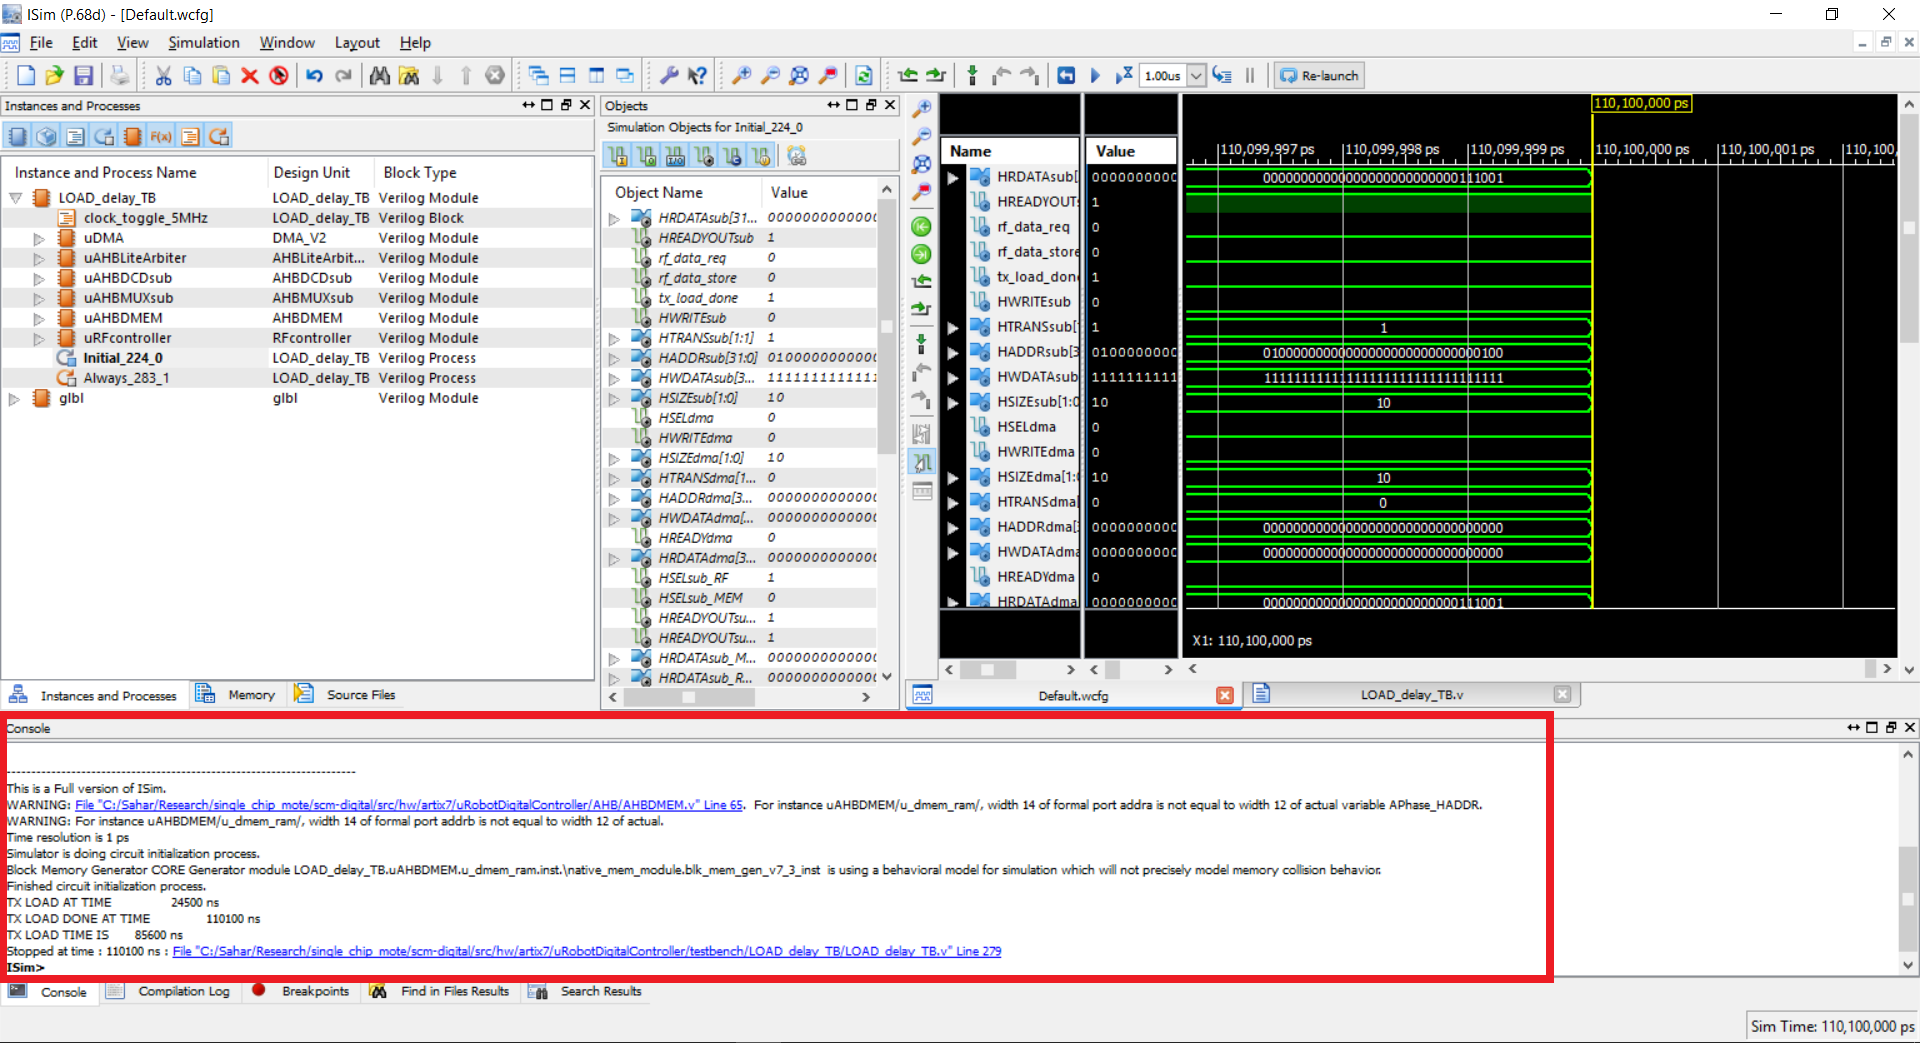
\includegraphics[width=1\linewidth]{isim-waveform0}
	\caption{ISim window after launching a simulation using the default wave configuration file}
	\label{fig:isim-waveform0}
\end{figure}
\begin{figure}
	\centering
	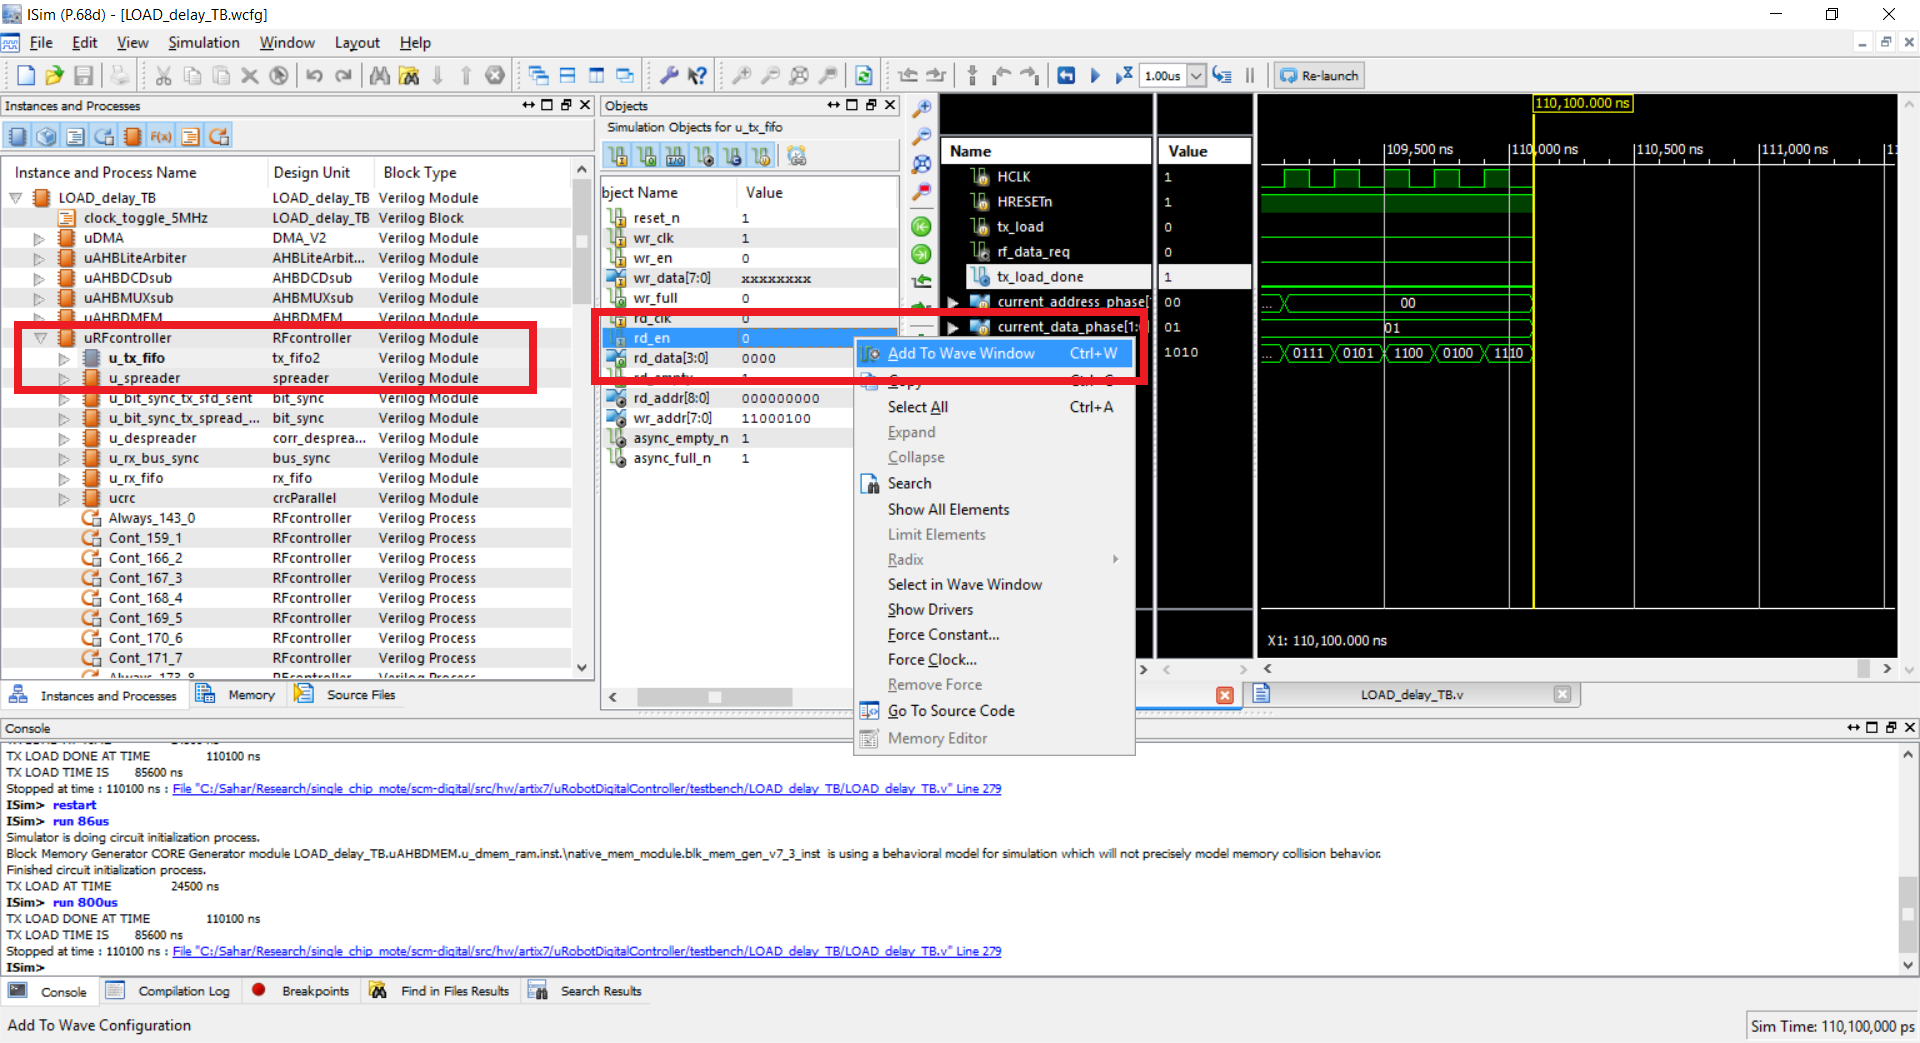
\includegraphics[width=1\linewidth]{isim-waveform1}
	\caption{Adding a signal to the waveform window in ISim}
	\label{fig:isim-waveform1}
\end{figure}
\begin{figure}
	\centering
	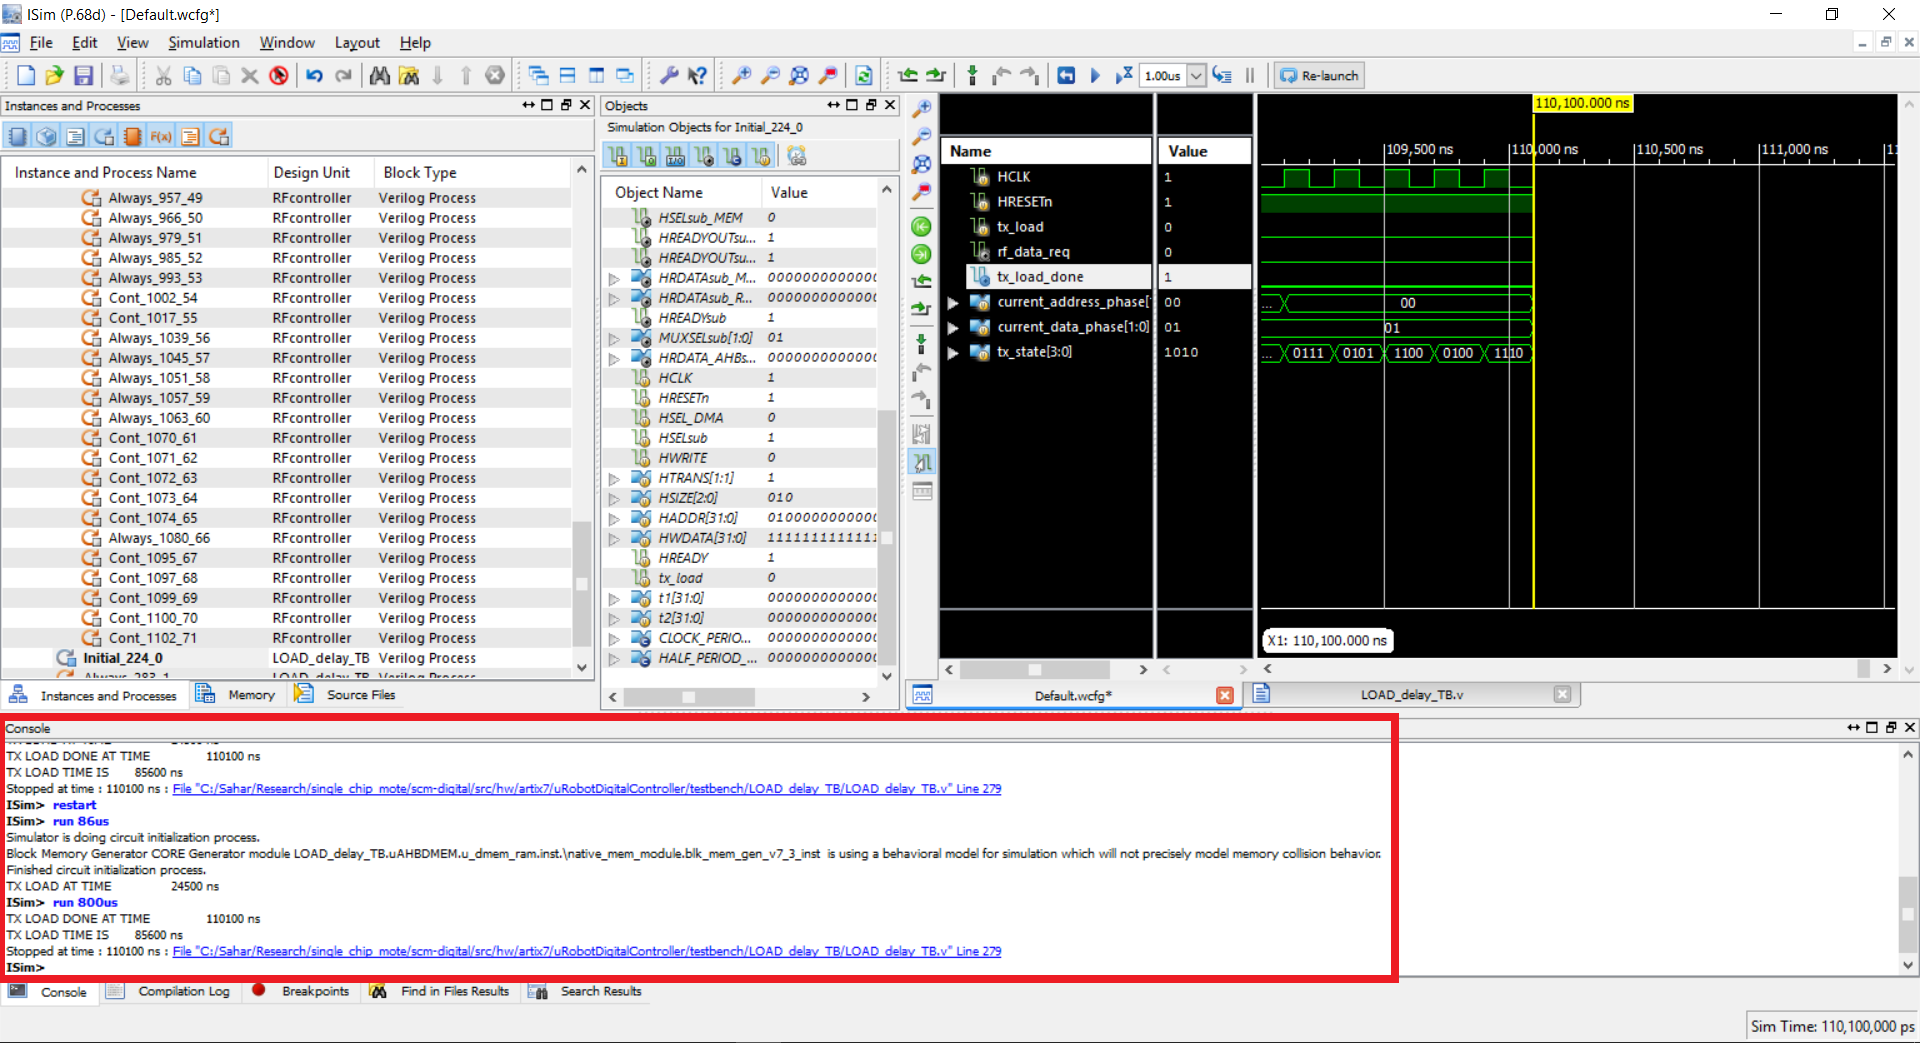
\includegraphics[width=1\linewidth]{isim-waveform2}
	\caption{Restarting and running a simulation in ISim}
	\label{fig:isim-waveform2}
\end{figure}
\begin{figure}
	\centering
	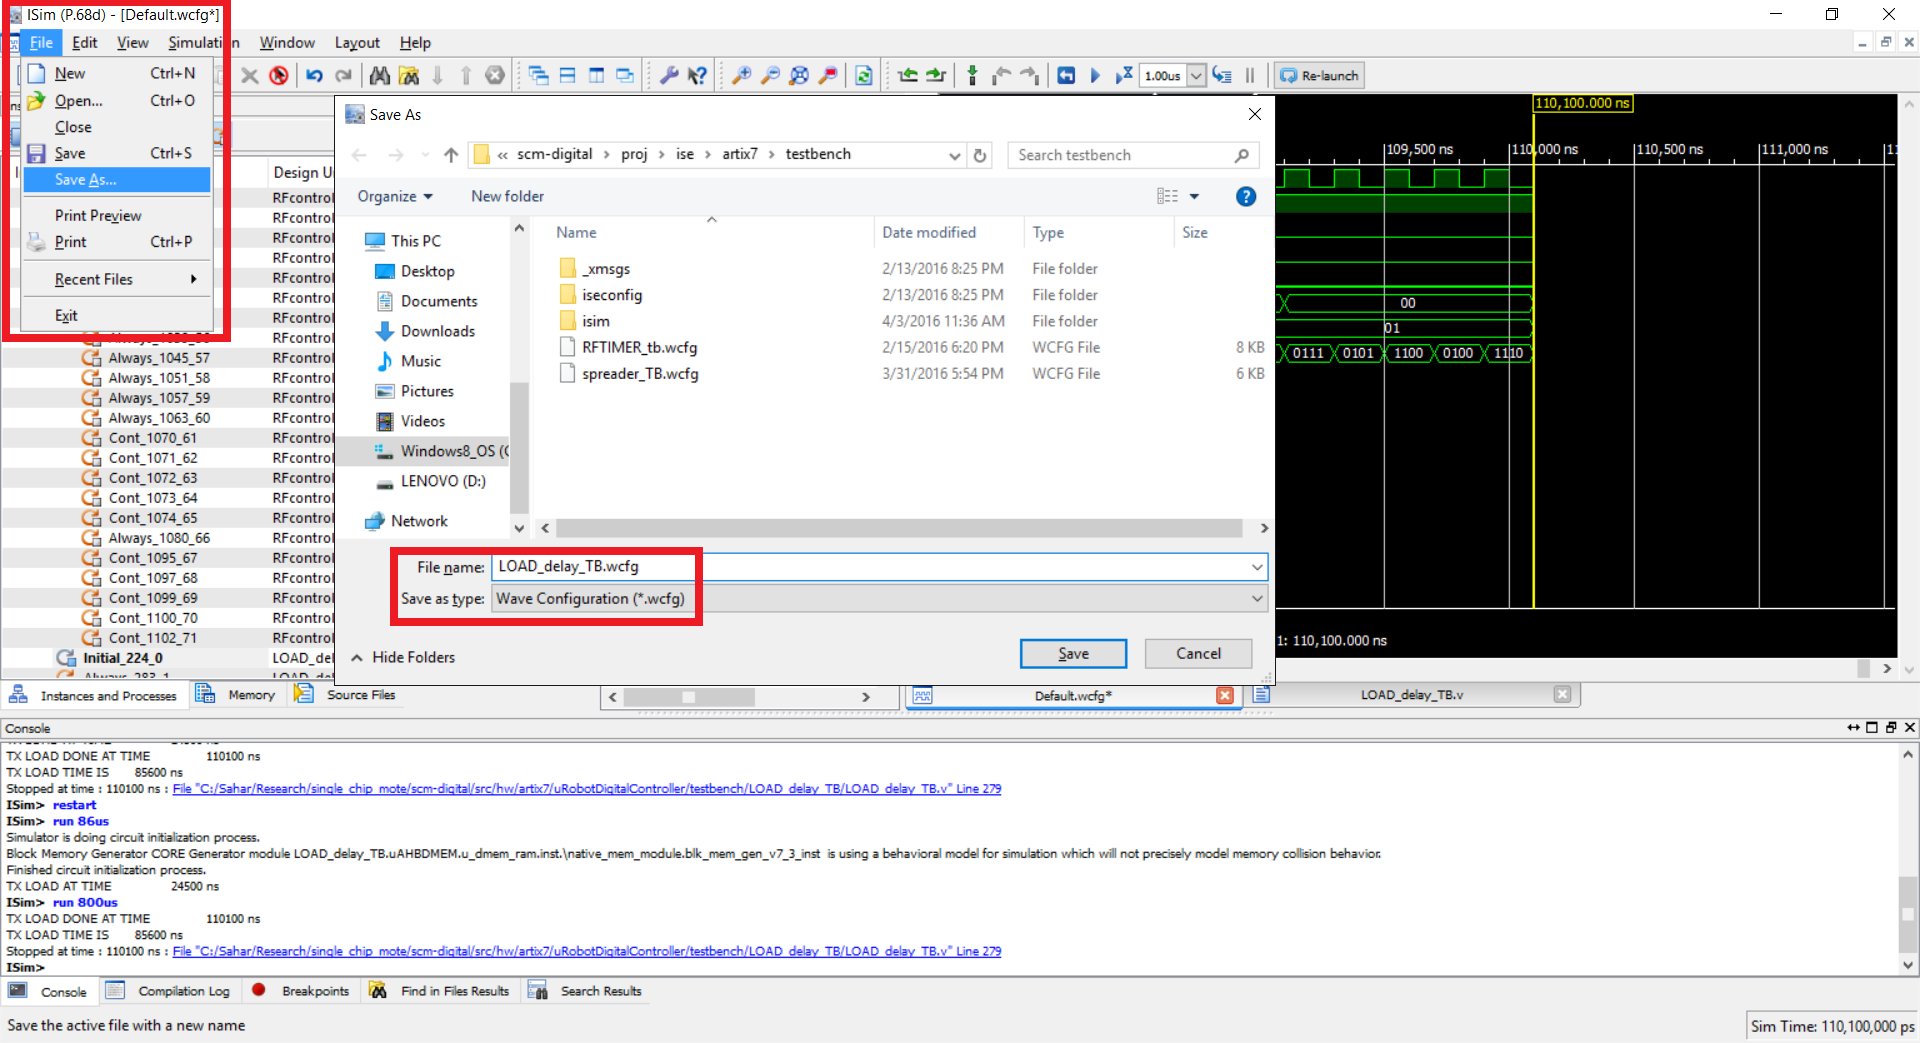
\includegraphics[width=1\linewidth]{isim-waveform3}
	\caption{Saving a wave configuration file in ISim}
	\label{fig:isim-waveform3}
\end{figure}

\section{Real-Time Testing on FPGA}
Testbenches are useful when determining that a module behaves as according to its specification in an ideal environment. The main limitation with testbenches is that they fail to uncover bugs in edge cases that are not considered or expected by the designer. Running real-time integration tests reveal problems where modules interact with one another and assumptions about interfaces break down. Test software can also indicate situations where the module fails to satisfy the requirements for the application, or the hardware does not behave according to what the software developer expects. Modules that interact with circuits and signals from outside the digital system, such as the ADC or the radio, should also be verified in real-time, in order to ensure that the digital and analog circuits interact appropriately and that the digital module can handle any non-idealities that inevitably come from a noisy system.

\subsection{Test Programs}
Testing the Single Chip Mote digital system on an FPGA will require a C program compiled for the Cortex-M0. Ideally this program would also contain code to exercise all of the features that require testing, including code to check if the results are as expected.

The current demo code found in \texttt{scm-digital/proj/keil/uRobotDigitalCon\-t\-r\-oller/code.uvprojx} is not an exhaustive test suite; however, it does exercise many of the features of the radio controller and radio timer, and is typically used to verify that minor changes to those modules have not caused them to stop working outright. This code is also not the best test code since it requires user input via UART.

In the future, an autonomous test suite should be developed to provide stimulus to each Single Chip Mote peripheral, and check if the outputs match expectation, and then either send the results over UART or toggle the general-purpose outputs to indicate when the test finishes and if it is a success or failure. This test suite would then be run after hardware changes and hardware testbenches.

\subsection{ChipScope}
Unexpected behavior encountered during FPGA testing is much more difficult to diagnose than in simulation. Simulations allow the designer to observe and sometimes manipulate signals and state within a design and work quickly and iteratively to resolve the issue. Within an FPGA, these signals and states are inaccessible, and it is not possible to `pause' a circuit in order to examine its state. Xilinx does provide a tool called ChipScope, which is used to probe and measure internal FPGA signals and registers in real-time. A designer can choose which signals to probe after running the Synthesis process, and before running the Translate process. Any changes to the probed signals will require running the Translate, Map, and Place \& Route processes again. For more information on how to use ChipScope, see the following tutorial from Xilinx: Using Xilinx ChipScope Pro ILA Core with Project Navigator to Debug FPGA Applications \cite{chipscope-pro-tutorial}. A copy is found in \path{scm-digital/doc}.

The recommended debugging process using ChipScope is as follows:

\begin{enumerate}
	\item Determine which module may be causing the erroneous behavior.
	\item Make an educated guess about which signals and state in that module may reveal the source of the erroneous behavior, and connect those signals to the ChipScope ILA unit.
	\item Run through the processes to generate a bitstream for the design, and load the bitstream using the ChipScope Pro software.
	\item Set up the trigger settings to capture the erroneous behavior.
	\item If there is no trigger or the captured data does not reveal the erroneous behavior, modify the trigger settings or add more signals to the ILA and try again.
	\item Once the problem is detected, use the captured data to determine the possible bug in the Verilog code that would lead to the erroneous behavior. It also may be possible use the captured data to replicate the situation in a testbench for further debugging.
	\item Update the code with a possible fix.
	\item Test the new code in real-time or in simulation and determine if the problem is solved. It may be necessary to repeat the previous step multiple times before a solution is found.
\end{enumerate}

Note that ChipScope ILA units use up a considerable amount of block RAM resources  on the FPGA, and it is possible to create an ILA unit that requires more RAM than available due to the number of signals that are sampled. In this case the Map process will fail and the ILA unit must be modified to sample fewer signals.